\clearpage \section{Models}

\label{chap:models}

One crucial step is the splitting of the dataset into test and training data. According to best practices, the splits can range from 60\% to 40\% until 80\% to 20\%. In this thesis, the test dataset contains the last nine matchdays of the 2020/2021 Bundesliga season, i.e., the matchdays 26 to 34. This distribution represents a 70:30 split.

Before the models can be implemented, a metric has to be found for comparing the models. For machine learning problems, it is helpful to define a metric beyond the usual metrics that make the models' predictions comparable to the desired outcome. Reflecting on the considerations from the Business Context chapter \ref{chap:business_context}, the realistic goal of the models should be to predict players' performances accurately enough to regularly produce a line-up that achieves a score of 65\% of the best possible score. By reaching this goal, the models would be able to win a prize now and then. For this reason, the following two own metrics are created. The first metric measures the percentage of points achieved by the model compared to the best possible score. The second metric takes the first metric to calculate the prize money earned in case of reaching the winning zone.

In order for the first metric to be measured, the best line-up must be calculated for each matchday in the test dataset. Therefore, the achieved score from each player for each matchday is taken and decreased by their current transfer market value according to equation (\ref{eq:player_score_with_value}) to get the \textbf{adjusted player score} \emph{S\textsubscript{P\textsubscript{i}M}}. Using these values, the best line-up can be assembled by taking the corresponding number of best players for each position for each available line-up and adding up their scores. The resulting sum is the highest possible score that can be achieved for each formation. The formation with the most points is the best possible line-up, which corresponds to 100\% for the first metric. The percentage of points for the team set up by the model is then calculated by dividing the resulting score by the best possible score. This metric is called the \textbf{percentage of best possible score} \emph{S\textsubscript{LM\%}}.

For the second metric, as SPITCH, unfortunately, does not give any insight into the exact calculation of the prize money within the profit zone, a formula has to be created using the available data, which represents this calculation as closely as possible. Due to the lack of data, conscientious simplifications have to be made. Like already mentioned in the chapter \emph{Business Context}, the best ranks usually achieve 80 to 85\% of the maximum possible score. Accordingly, in the simplified calculation of the price, the first place is won as soon as S\textsubscript{LM\%} is 80\% or above. Every percent less means one place further down in the ranking. Thus, the \emph{Rank} can be calculated from \emph{S\textsubscript{LM\%}} using the equation:

\begin{equation}
    Rank = \frac{0.81 - S\textsubscript{LM\%}}{0.01} 
    \label{eq:percentage_of_best_score_to_rank}
\end{equation}

The corresponding prize to each rank can be seen on the screenshot from \emph{SPITCH} in figure \ref{fig:prize-percentage}.

\begin{figure}[H]
    \centering
    \fbox{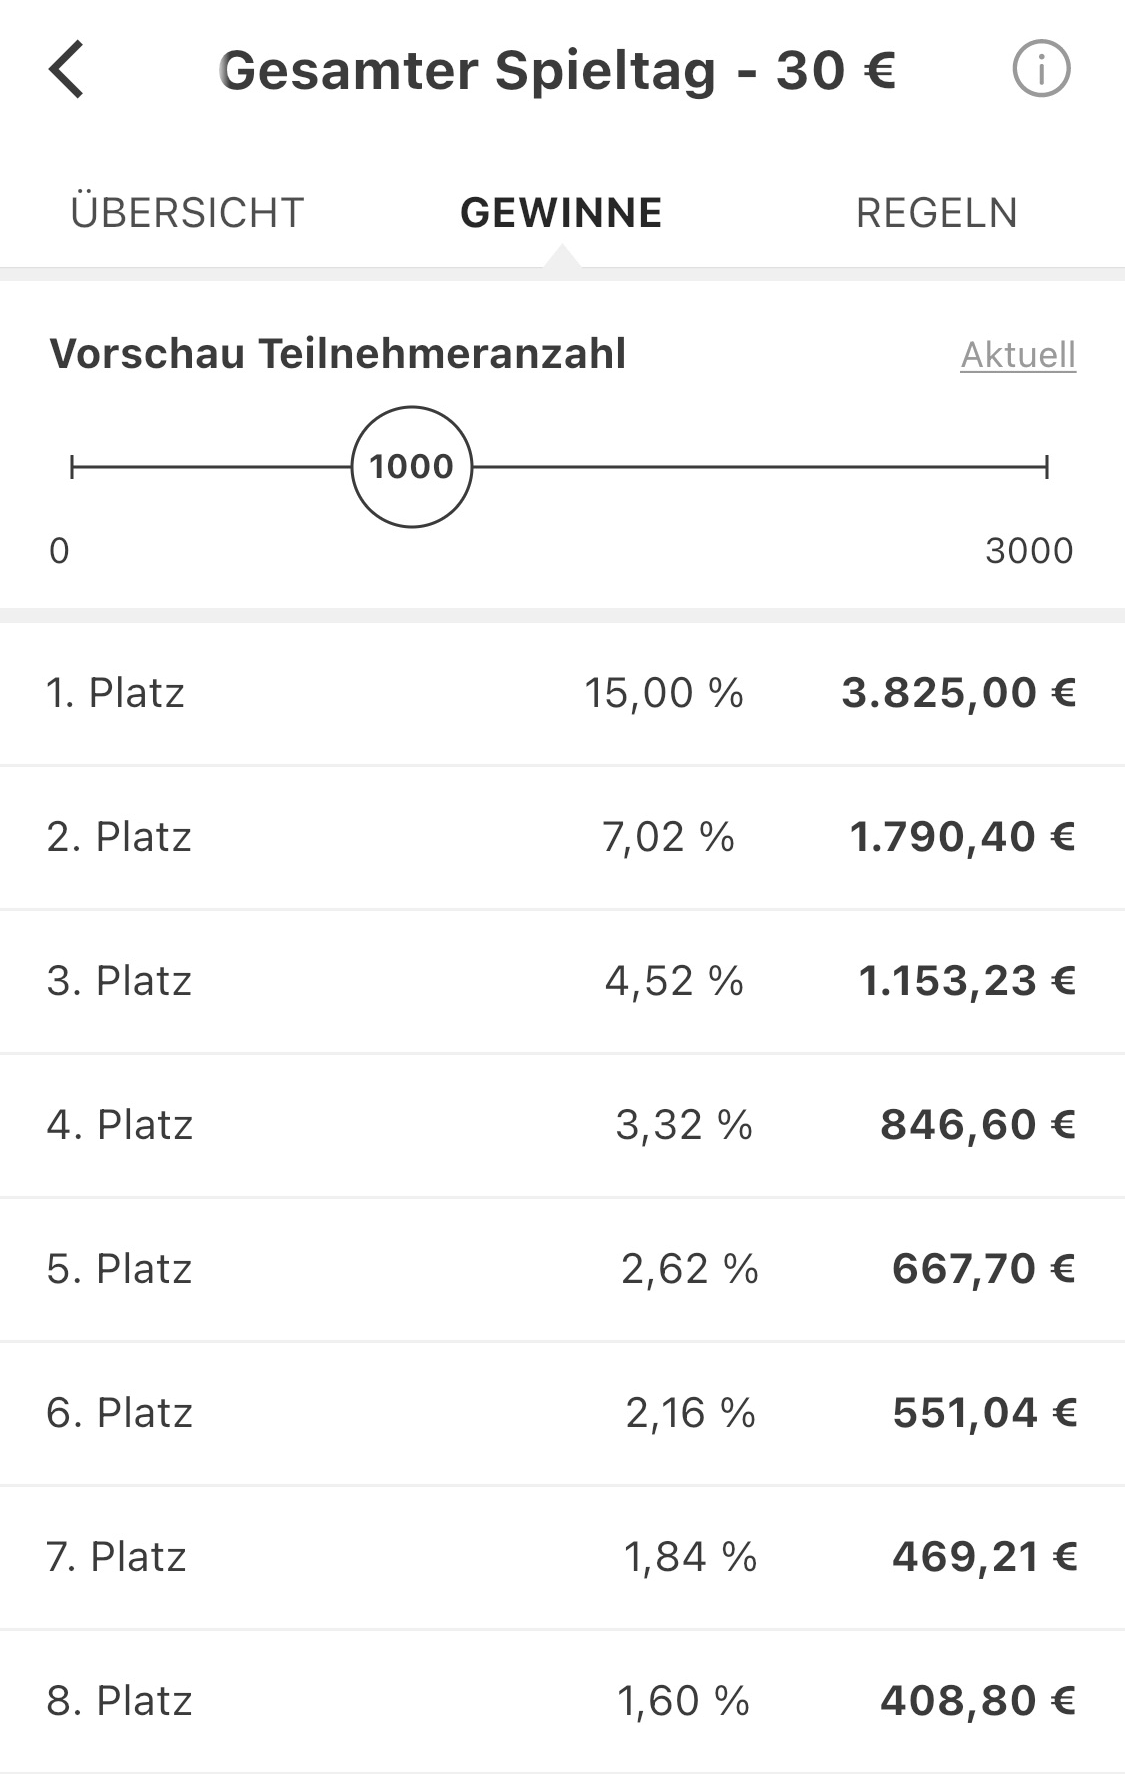
\includegraphics[width=6cm]{chapter/4_implementation/figures/ranking_percentage.png}}
    \captionsetup{justification=centering}
    \caption{Percentage of Prize per Rank for the €30 Pitch}
    \label{fig:prize-percentage}
\end{figure}

This distribution applies to all \emph{pitches} with stakes. The following function can be derived using the data from this screenshot, which calculates the share of the profit \emph{Profit\textsubscript{\%}} from the associated rank \emph{Rank}:

\begin{equation}
    Profit\textsubscript{\%} = 27.56 * \emph{e}^{-0.72 * Rank} + 1.3 
    \label{eq:rank_to_profit}
\end{equation}

The prize money consists of the players' stakes and therefore is the product from participants and stake. For the evaluation, the models attend the €2 pitch with \numprint{1000} participants. Thus, the prize money equals €\numprint{2000} each round.

Before the machine learning models are created, two \emph{dummy} models are defined. These models serve as comparisons and represent alternative strategies. The first model randomly assembles a line-up and is called \emph{guess}. The second model fields the best line-up from the previous matchday for the upcoming matchday and is called \emph{previous best}. The table below presents the results of these models, ordered by their performance on \emph{Mean S\textsubscript{LM\%}}:

\begin{table}[H]
    \renewcommand{\arraystretch}{1.0}
    \caption{Dummy Models Results}
    \label{tab:results_of_dummy_models}
    \begin{tabular}{@{}cccccc@{}}
    \toprule
    \textbf{Design} & \textbf{Model} & \textbf{Mean S\textsubscript{LM\%}} & \textbf{MAE of \^{S}\textsubscript{P\textsubscript{i}}} & \textbf{Prize Money} & \textbf{\# Prizes Won} \\ \midrule
    dummy   & previous best & 0.4133 & 197.45 & -€18 & 0 \\
    dummy   & guess         & 0.3511 & 197.18 & -€18 & 0 \\ \bottomrule
    \end{tabular}
\end{table}

The results show that the model \emph{previous best} performs with a mean of 41.33\% of the best possible score and therefore performs better than the model \emph{guess}. This result is no surprise, considering the strong autocorrelation of the player scores shown in the Data Exploration section \ref{chap:data_exploration}, indicating that players who recently performed well will most likely perform well in the future. However, although the model has set up better line-ups, it has a higher mean absolute error per player (MAE of \^{S}\textsubscript{P\textsubscript{i}}). Both models fail to win a prize, losing nine times €2, which equals a net loss of €18.

The results of the dummy models are now compared with the machine learning models available in the \emph{scikit-learn} Python package. The selection of regression models follows the results of the literature review. For this reason, these models are \emph{Multiple Linear Regression, Logistic Regression, Decision Trees, Random Forests, K-Nearest Neighbors, and Support Vector Machines}. Each model exists twice, once in \emph{baseline} and once in \emph{treatment} design. The treatment models have access to the betting odds data while the baseline models don't. All models are cross-validated with five stratified folds on the training dataset to minimize the bias in the accuracy scores of the models. The following table shows the results of the cross-validation, sorted by the MAE of \^{S}\textsubscript{P\textsubscript{i}}.

\begin{table}[H]
    \renewcommand{\arraystretch}{1.0}
    \setlength{\tabcolsep}{15pt}
    \centering
    \caption{Cross-Validation Results}
    \label{tab:cv_results}
    \begin{tabularx}{\textwidth}{lXr}
    \toprule
    \textbf{Design} & \textbf{Model} & \textbf{MAE of \^{S}\textsubscript{P\textsubscript{i}}} \\ \midrule
    treatment   & Multiple Linear Regression    & 99.32 \\
    baseline    & Multiple Linear Regression    & 99.73 \\
    treatment   & Random Forest Regression      & 102.95 \\
    treatment   & K-Nearest Neighbors           & 105.41 \\
    baseline    & K-Nearest Neighbors           & 106.38 \\
    baseline    & Random Forest Regression      & 107.55 \\
    treatment   & Logistic Regression           & 117.82 \\
    baseline    & Logistic Regression           & 118.52 \\
    treatment   & Support Vector Machines       & 120.06 \\
    baseline    & Support Vector Machines       & 120.52 \\
    baseline    & Decision Tree Regression      & 132.91 \\
    treatment   & Decision Tree Regression      & 135.91 \\
    dummy       & guess                         & 197.18 \\
    dummy       & previous best                 & 197.45 \\ \bottomrule
    \end{tabularx}
\end{table}

Three findings emerge from the results of the cross-validation. The first finding is that five of the six machine learning models provide more accurate predictions when accessing the betting odds. The second finding is that even the worst-performing machine learning model has a much smaller MAE than the dummy models. Therefore, machine learning algorithms seem to offer a predictive value in general. The last finding is that \emph{Multiple Linear Regression} and \emph{Random Forest Regression} are the two most accurate machine learning models. However, the models so far have only used their default parameters. Through a process called \textbf{hyperparameter tuning}, the models can improve even further. This procedure is applied in the next paragraph to the two previously mentioned most accurate models.

\emph{Multiple Linear Regression} and \emph{Random Forest Regression} differ in their complexity. While the former has only three Boolean parameters that can be optimized, \emph{Random Forest Regression} has more than ten parameters, most of which are numerical. Furthermore, two out of three of the linear regression parameters are unsuitable for optimization in this case. The parameters \emph{normalize} and \emph{positive} are dropped since the data has already been standardized, and there are features in the dataset such as betting odds where one feature at least must be negative. The only optimization parameter remaining is \emph{fit\_intercept}, which allows the regression to be calculated with or without an interception. This parameter did not make the models more precise. \\
The hyperparameter tuning of the Random Forest Regression Model happens with the six most influential parameters. Since four of these parameters can be any natural number, the Python packages called \emph{RandomizedSearchCV} and \emph{GridSearchCV} are used. Each of these packages takes a list of possible parameter settings and fits the models with different combinations from these parameter settings using cross-validation. \emph{GridSearchCV} takes all parameters and tests every possible combination, whereas \emph{RandomizedSearchCV} takes number ranges and randomly tests a pre-defined quantity of combination. Therefore, \emph{RandomizedSearchCV} narrows down the optimal parameter settings, and \emph{GridSearchCV} finds the optimal parameters in the narrowed down area afterward. Through this procedure, the following optimal parameters for the Random Forest Regression are found, resulting in the hyperparameter-tuned model:

 \begin{verbatim}
    RandomForestRegressor(max_depth=13,max_features='sqrt',bootstrap=True,
    min_samples_leaf = 9, min_samples_split = 2, n_estimators = 300)
 \end{verbatim}

 This model reaches the lowest MAE of \textbf{98.14} and thus predicts most accurately.

 After all the models have been created, fitted, and cross-validated, they can finally be used on the test dataset. The following table presents the results, ordered by their performance on \emph{Mean S\textsubscript{LM\%}}:

 \begin{table}[H]
    \renewcommand{\arraystretch}{1.0}
    \setlength{\tabcolsep}{6pt}
    \caption{Models' Results on the Test Dataset}
    \label{tab:results_test_data}
    \resizebox{\textwidth}{!}} & \textbf{MAE of \^{S}\textsubscript{P\textsubscript{i}}} & \textbf{Prize Money} & \textbf{\# Prizes Won} \\ \midrule
    treatment   & Tuned Random Forest Regression    & 0.5189 & 104.56 & €33.86     & 2 \\
    baseline    & Tuned Random Forest Regression    & 0.4922 & 104.92 & -€18.00    & 0 \\
    treatment   & Multiple Linear Regression        & 0.4911 & 105.28 & €8.01      & 1 \\
    baseline    & Random Forest Regression          & 0.4733 & 114.06 & -€18.00    & 0 \\
    treatment   & Random Forest Regression          & 0.4700 & 108.81 & -€18.00    & 0 \\
    baseline    & Multiple Linear Regression        & 0.4667 & 105.56 & -€18.00    & 0 \\
    baseline    & K-Nearest Neighbors               & 0.4489 & 111.81 & -€18.00    & 0 \\
    treatment   & K-Nearest Neighbors               & 0.4344 & 113.11 & -€18.00    & 0 \\
    dummy       & previous best                     & 0.4133 & 197.45 & -€18.00    & 0 \\
    baseline    & Decision Tree Regression          & 0.3922 & 141.60 & -€18.00    & 0 \\
    treatment   & Logistic Regression               & 0.3867 & 123.85 & -€18.00    & 0 \\
    baseline    & Logistic Regression               & 0.3811 & 123.95 & -€18.00    & 0 \\
    treatment   & Decision Tree Regression          & 0.3556 & 145.67 & -€18.00    & 0 \\
    dummy       & guess                             & 0.3511 & 197.18 & -€18.00    & 0 \\
    treatment   & Support Vector Machines           & 0.3400 & 126.94 & -€18.00    & 0 \\
    baseline    & Support Vector Machines           & 0.3344 & 127.16 & -€18.00    & 0 \\\bottomrule
    \end{tabular}
    }
\end{table}

The table shows that the \textbf{hyperparameter tuned random forest regression model} in the treatment design, i.e., with the betting odds as features, made the \textbf{most accurate predictions} on the test dataset, with an average of just under \textbf{52\%} of the points from the best possible line-up. The model is 16\%, or 11\% respectively, better than the dummy models. On average, the model misjudged each player by 104.5 points in the test and is thus 6 points worse than on the training dataset. If the winning zone would start at 60\% of the best possible score, the model would have \textbf{won a prize two times} and brought in total prize money of \textbf{33.86€}. This profit is possible because the standard deviation of the best model is 7.6\%, which indicates that it is quite realistic for the model to reach more than 60\% in nine tries.

\clearpage Interestingly, although the multiple linear regression model in the treatment design made less accurate predictions on average than the random forest regression model in the baseline design, it still won a prize. This means that despite poorer individual predictions, it lined up a better team, probably because of luck.

Furthermore, it is noticeable that on the test dataset, only four out of seven models performed better in the treatment design than in the baseline design. This could indicate that the models were overfitted on the betting odds in the training dataset. However, the influence of the betting odds will be examined in detail in the next section.






